%==============================================================================
%== template for LATEX poster =================================================
%==============================================================================
%
%--A0 beamer slide-------------------------------------------------------------
\documentclass[final]{beamer}
\usepackage{etex} % too many packages in beamerposter
\usepackage[orientation=portrait,size=a0,
            scale=1.4         % font scale factor
           ]{beamerposter}

\usepackage{booktabs}
\usepackage{wrapfig}
\geometry{
  hmargin=2.5cm, % little modification of margins
}

%
\usepackage[utf8]{inputenc}
\graphicspath{{figures/}} % Location of the graphics files
\newcommand{\abnet}{{\sc ABnet}}
\newcommand{\norm}[1]{\lVert#1\rVert}
\newcommand{\tup}[1]{\langle#1\rangle}

\linespread{1.05} %%% TODO CHANGE (was 1.15)
%
%==The poster style============================================================
\usetheme{sharelatex}

%==Title, date and authors of the poster=======================================
\title
[Interspeech (2015, Dresden, Germany)] % Conference
{ % Poster title
Hybrid Spoken Term Discovery-ABnet System\\
Finding words to learn segments
}

\author{ % Authors
Roland Thiolli\`ere\inst{*}, Ewan Dunbar\inst{*}, Gabriel Synnaeve\inst{*\dagger}, Maarten Versteegh\inst{*}, Emmanuel Dupoux\inst{*}
}
\institute
[ENS] % General University
{
\inst{*} LSCP, \'{E}cole Normale Sup\'{e}rieure / EHESS / CNRS, Paris, France\\%[0.3ex]
\inst{\dagger} now at Facebook AI Research\\[0.5ex]
\inst{} \begin{small}\texttt{rolthiolliere@gmail.com, emd@umd.edu, gabrielsynnaeve@gmail.com, maartenversteegh@gmail.com, emmanuel.dupoux@gmail.com}\end{small}
}
%\date{\today}


\begin{document}
\begin{frame}[t]
%==============================================================================
\begin{multicols}{2} % try 2
%==============================================================================
%==The poster content==========================================================
%==============================================================================

\section{Introduction}

\begin{itemize}
\item This system is the combination of two architectures: a \textbf{spoken term discovery}\cite{jansenvandurme2011} (STD) and a \textbf{siamese neural network}\cite{synnaevedupoux2014} (\abnet{}).
\item The STD system finds matching patterns in the acoustic signal.
\item The \abnet{} is trained to minimize the distance between those matching patterns, and maximize the distance between non matching patterns.
\end{itemize}


%-----------------------------------------
%	Motivation
%-----------------------------------------

\section{Motivation}

The high level idea: It is easier to discriminate words than phonemes → \textbf{use Track 2 to help with Track 1}.

%-----------------------------------------
%       SYSTEM
%-----------------------------------------

\section{System}

%\vspace{0.5cm}
\begin{figure}[ht!]
  \begin{center}
    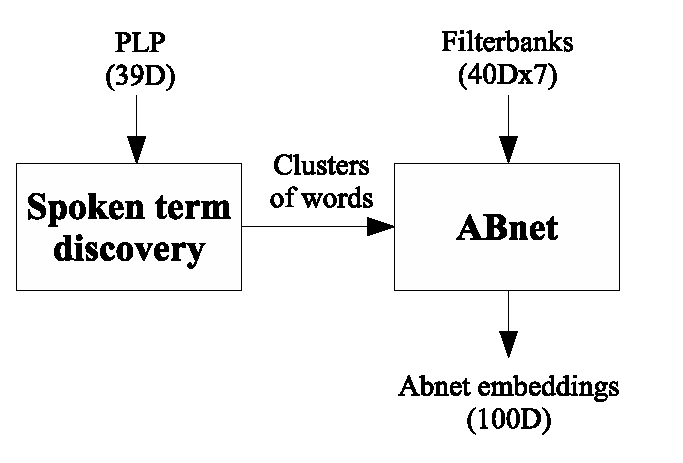
\includegraphics[width=0.7\columnwidth]{system_overview2}
    \caption{\label{fig:system}Overview of the components of our system.}
  \end{center}
\end{figure}

%-----------------------------------------
%       SPOKEN TERM DISCOVERY
%-----------------------------------------

\subsection{Spoken term discovery}

\begin{multicols}{2} % try 2

\begin{figure}
  \begin{center}
    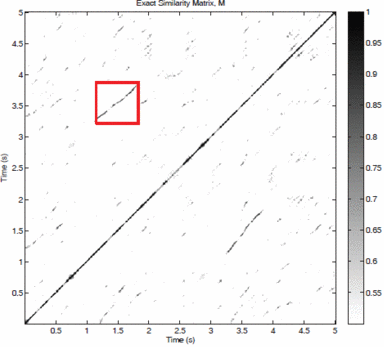
\includegraphics[width=0.6\columnwidth]{similarity_matrix}
  \end{center}
  \caption{\label{fig:system}Similarity matrix of the signal. Source: \cite{jansenvandurme2011}}
\end{figure}
\columnbreak

\begin{itemize}
\item System used as baseline for track 2 \cite{versteeghetal2015}.
\item Computes an approximation of the similarity matrix (cosine similarity).
\item Searches for diagonal patterns
\item Filters and cluster those patterns
\end{itemize}
See \cite{jansenvandurme2011} for more.

\end{multicols}

% \begin{minipage}[t]{0.45\columnwidth}
% \begin{figure}
%   \begin{center}
%     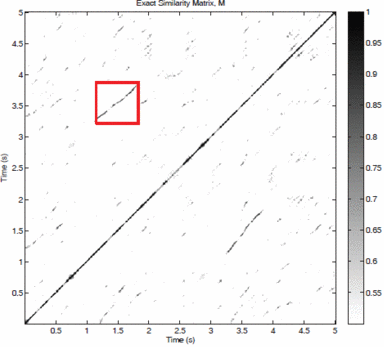
\includegraphics[width=0.2\columnwidth]{similarity_matrix}
%   \end{center}
%   \caption{\label{fig:system}Similarity matrix of the signal. Source: \cite{jansenvandurme2011}}
% \end{figure}
% \end{minipage}

\subsection{ABnet}

\begin{itemize}
\item The \abnet{} is a siamese neural network architecture: the weights in the second branch are the duplicate of the weights in the first branch.
\item It learns a space where inputs with the same label are close together, and inputs with different labels are far apart. 
\item Input: a pair of examples (A, B) and a label Y=(same|different), here 7 stacked frames of 40 dimensionnal filterbanks.
\item loss function = similarity if same, distance if different.

\columnbreak
\vspace{1cm}
\begin{figure}[ht!]
  \begin{center}
    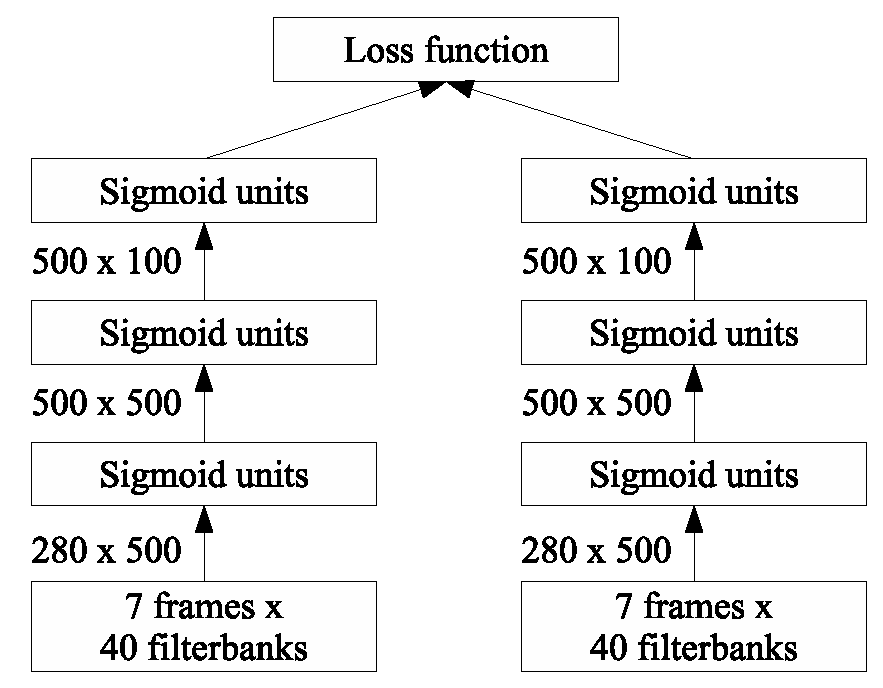
\includegraphics[width=0.65\columnwidth]{abnet}
    \caption{\label{fig:system}Overview of the components of our system.}
  \end{center}
\end{figure}

\item Loss function used:
\begin{small}
\[
\mathcal{L}(A, B) =
\begin{cases}
(1-\cos(Y_A, Y_B)) / 2 & \text{if same} \\
\cos^2(Y_A, Y_B)       & \text{if different}
\end{cases}
\]
\end{small}
\item Pairs of ``different'' words are randomly selected amongst the discovered patterns. Pairs of same words are DTW aligned.
\item Pairs of same/different words → pairs of same/different frames
% \noindent        
% where $$\cos(x, y) = \frac{\tup{x, y}}{\norm{x}\norm{y}}$$

\end{itemize}

% \subsection{Speaker embedding}

% Adding speaker information.

% \begin{figure}[ht!]
%   \begin{center}
%     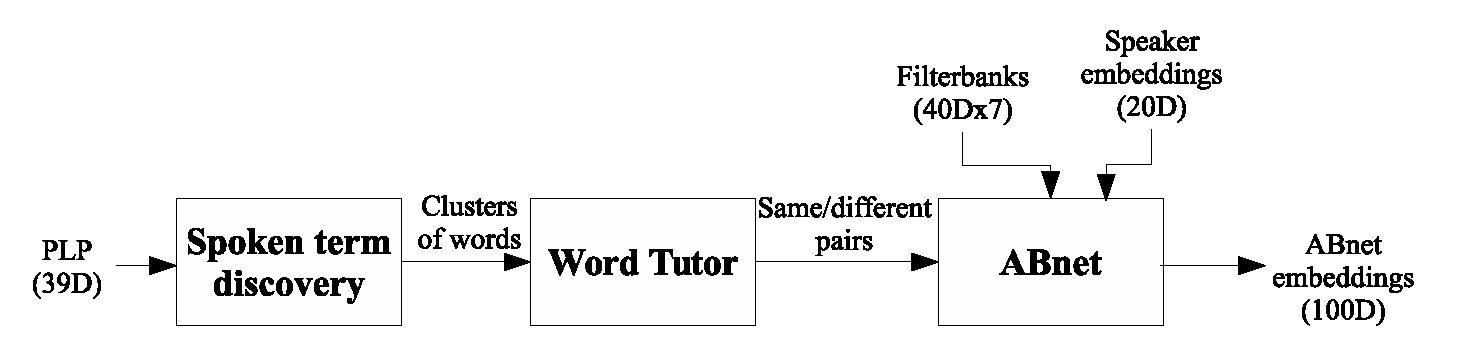
\includegraphics[width=\columnwidth]{system_spk}
%     \caption{\label{fig:system}Overview of the components of our system.}
%   \end{center}
% \end{figure}


%----------------------------------------------------------------------------------------
%	RESULTS 
%----------------------------------------------------------------------------------------

\section{Results}

\begin{table}[h]
\caption{\label{tab:std-stats} Evaluation of the STD system. These fragments serve as input to the \abnet{}.}
\small
% \begin{tabular}{lccccccccccccccccc}
\begin{tabular}{lccccc}
\hline
         & Words & Pairs & Classes & NED   & Coverage \\
\hline
English & 6512 & 4305 & 3149 & 0.219 & 0.163 \\
\hline
Xitsonga & 3582 & 1818 & 1782 & 0.120 & 0.162 \\
\hline
\end{tabular}
\end{table}
\vspace{1cm}

\begin{itemize}
\item The speech representation is evaluated with the ABX paradigm (see \cite{versteeghetal2015}).
\item Two tasks: discriminate phones within speakers, and discriminate phones across speakers.

\begin{figure}[ht!]
  \begin{center}
    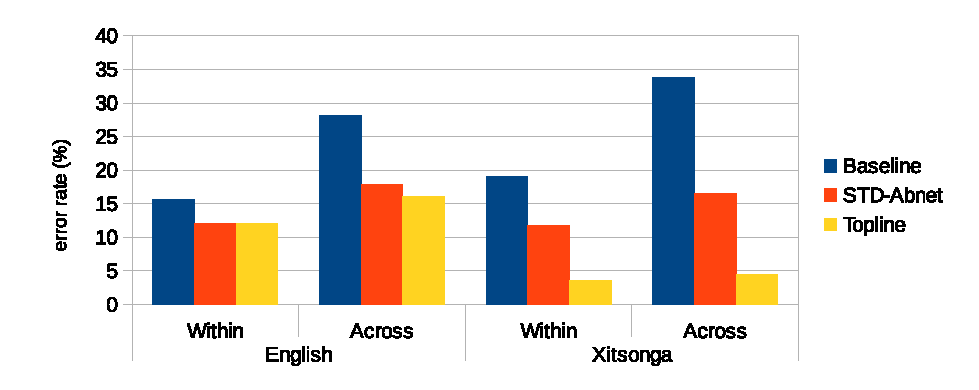
\includegraphics[width=0.8\columnwidth]{results}
    \caption{\label{fig:system}Within and across speaker Minimal Pair ABX error rates.}
  \end{center}
\end{figure}

%
% \vspace{1cm}
% \begin{table}[htb]
% \caption{ Within and across speaker Minimal Pair ABX error rates.}
% \label{tab:track1}
% \vspace{1cm}
% \centerline{
% \begin{tabular}{lcccc}
% \hline
%   & \multicolumn{2}{c}{\underline{English}}  & \multicolumn{2}{c}{\underline{Xitsonga}}    \\
%   & Within  & Across   & Within  & Across   \\
% \hline
%   Baseline (MFCC)          & \emph{15.6}      & \emph{28.1}      & \emph{19.1}      & \emph{33.8}      \\
%   Topline (HMM-GMM)           & \emph{12.1}      & \emph{16.0}      & \emph{3.5}       & \emph{4.5}      \\
% \hline
% STD $\rightarrow$ \abnet{} & \textbf{12.0}      & \textbf{17.9}      & \textbf{11.7}      & \textbf{16.6}      \\
% \hline
% \end{tabular}
% }
% \end{table}
%
\end{itemize}


%----------------------------------------------------------------------------------------
%	CONCLUSIONS
%----------------------------------------------------------------------------------------

% \color{SaddleBrown} % SaddleBrown color for the conclusions to make them stand out

\section{Conclusions}

\begin{itemize}
\item Despite the low number of examples, a good speech representation can be learnt.
\item Close to topline in english.
\item Forthcoming research: Loop over the system (STD on learnt features).
\end{itemize}

% \color{DarkSlateGray} % Set the color back to DarkSlateGray for the rest of the content

%----------------------------------------------------------------------------------------
%	FORTHCOMING RESEARCH
%----------------------------------------------------------------------------------------

%----------------------------------------------------------------------------------------
%	REFERENCES
%----------------------------------------------------------------------------------------

\subsection{References \& Acknowledgements}

\nocite{*} % Print all references regardless of whether they were cited in the poster or not
\bibliographystyle{IEEEtran} % Plain referencing style
\bibliography{bib} % Use the example bibliography file sample.bib

%----------------------------------------------------------------------------------------
%	ACKNOWLEDGEMENTS
%----------------------------------------------------------------------------------------

\vspace{1cm}
We would like to thank Aren Jansen for letting us use his spoken term discovery system pre-release, and for his technical support.
%----------------------------------------------------------------------------------------

%--End of references-----------------------------------------------------------

\end{multicols}

%==============================================================================
\end{frame}
\end{document}

